\documentclass[a4paper]{article}
\usepackage{titling}
\setlength{\droptitle}{-3em}
\usepackage{sectsty}
\usepackage{pdfpages}
\usepackage{graphicx}
\graphicspath{{img}}
\usepackage[a4paper]{geometry}
\usepackage{afterpage}
\usepackage{lipsum}
\usepackage{amsmath}
% \usepackage[defaultsans]{tgheros}
\renewcommand{\familydefault}{\sfdefault}
\usepackage{textcomp}
\usepackage{hyperref}
\hypersetup{
    colorlinks=true,
    linkcolor=blue,
    filecolor=magenta,      
    urlcolor=cyan,
    pdftitle={Overleaf Example},
    pdfpagemode=FullScreen,
  }
  
% Margins
% \topmargin=-0.45in
% \evensidemargin=0in
% \oddsidemargin=0in
% \textwidth=6.5in
% \textheight=9.0in
% \headsep=0.25in

\geometry{margin=0.6in}


\title{Breadboard Prototype \#1}
\author{William Vestergaard, Abel Nagy, Marta Borek}
\date{\today}

\begin{document}


\maketitle	
\section{Toy concept}

\noindent Our interactive toy concept is based on a popular game called \textit{Simon Says}, where users have to input a sequence of colored buttons provided with voice commands. We extend the original idea by providing the sequences in both visual (lighting LEDs) and haptic (buzzing disc motors) manner.


\noindent Target user group of our project is anyone interested in improving their concentration and short-term memory through tactile and visual means, but due to the high level of interactivity and the competitive nature of the game it might be particularly appealing for children (age group 10-13).

\section{Demo}
\href{https://aarhusuniversitet-my.sharepoint.com/:v:/g/personal/au802349_uni_au_dk/EYu93GnpKyVOjn9N1xiUcd0BokxDAjE5eCbD5Ibb2XIgbQ?nav=eyJyZWZlcnJhbEluZm8iOnsicmVmZXJyYWxBcHAiOiJPbmVEcml2ZUZvckJ1c2luZXNzIiwicmVmZXJyYWxBcHBQbGF0Zm9ybSI6IldlYiIsInJlZmVycmFsTW9kZSI6InZpZXciLCJyZWZlcnJhbFZpZXciOiJNeUZpbGVzTGlua0NvcHkifX0&e=tQ1Llt}{Link to the video}

\noindent Video shows the prototype output three sequences with the use of both buzzers and LEDs, each followed by user input and the final success/failure indication. Two first sequences are repeated correctly, resulting in a blinking green LED, signifying success. The third sequence input is incorrect, so it results in a failure indication, shown through the red LED.

\section{Circuit Diagram}
Our circuit diagram was drawn in Eagle from Fusion 360 with the use of custom component piece for ESP32.



\subsection{Color Coding}

\begin{itemize}
\item \textbf{yellow} - ESP32 C3 mini main controller.
\item \textbf{pink} - ATmega agent controlling LEDs (green) and their corresponding input buttons (left side of the image).
\item \textbf{cyan} - ATmega agent controlling buzzing motor discs (orange) and their corresponding input buttons (right side of the image).
\item \textbf{red} - Status indication LEDs.
\item \textbf{green} - LEDs.
\item \textbf{orange} - Buzzing disc motors.
\item \textbf{brown} - Step-up converter.
\item \textbf{olive green} - Step-down converter.
\item \textbf{purple} - Li Po 3.7V battery.
\end{itemize}


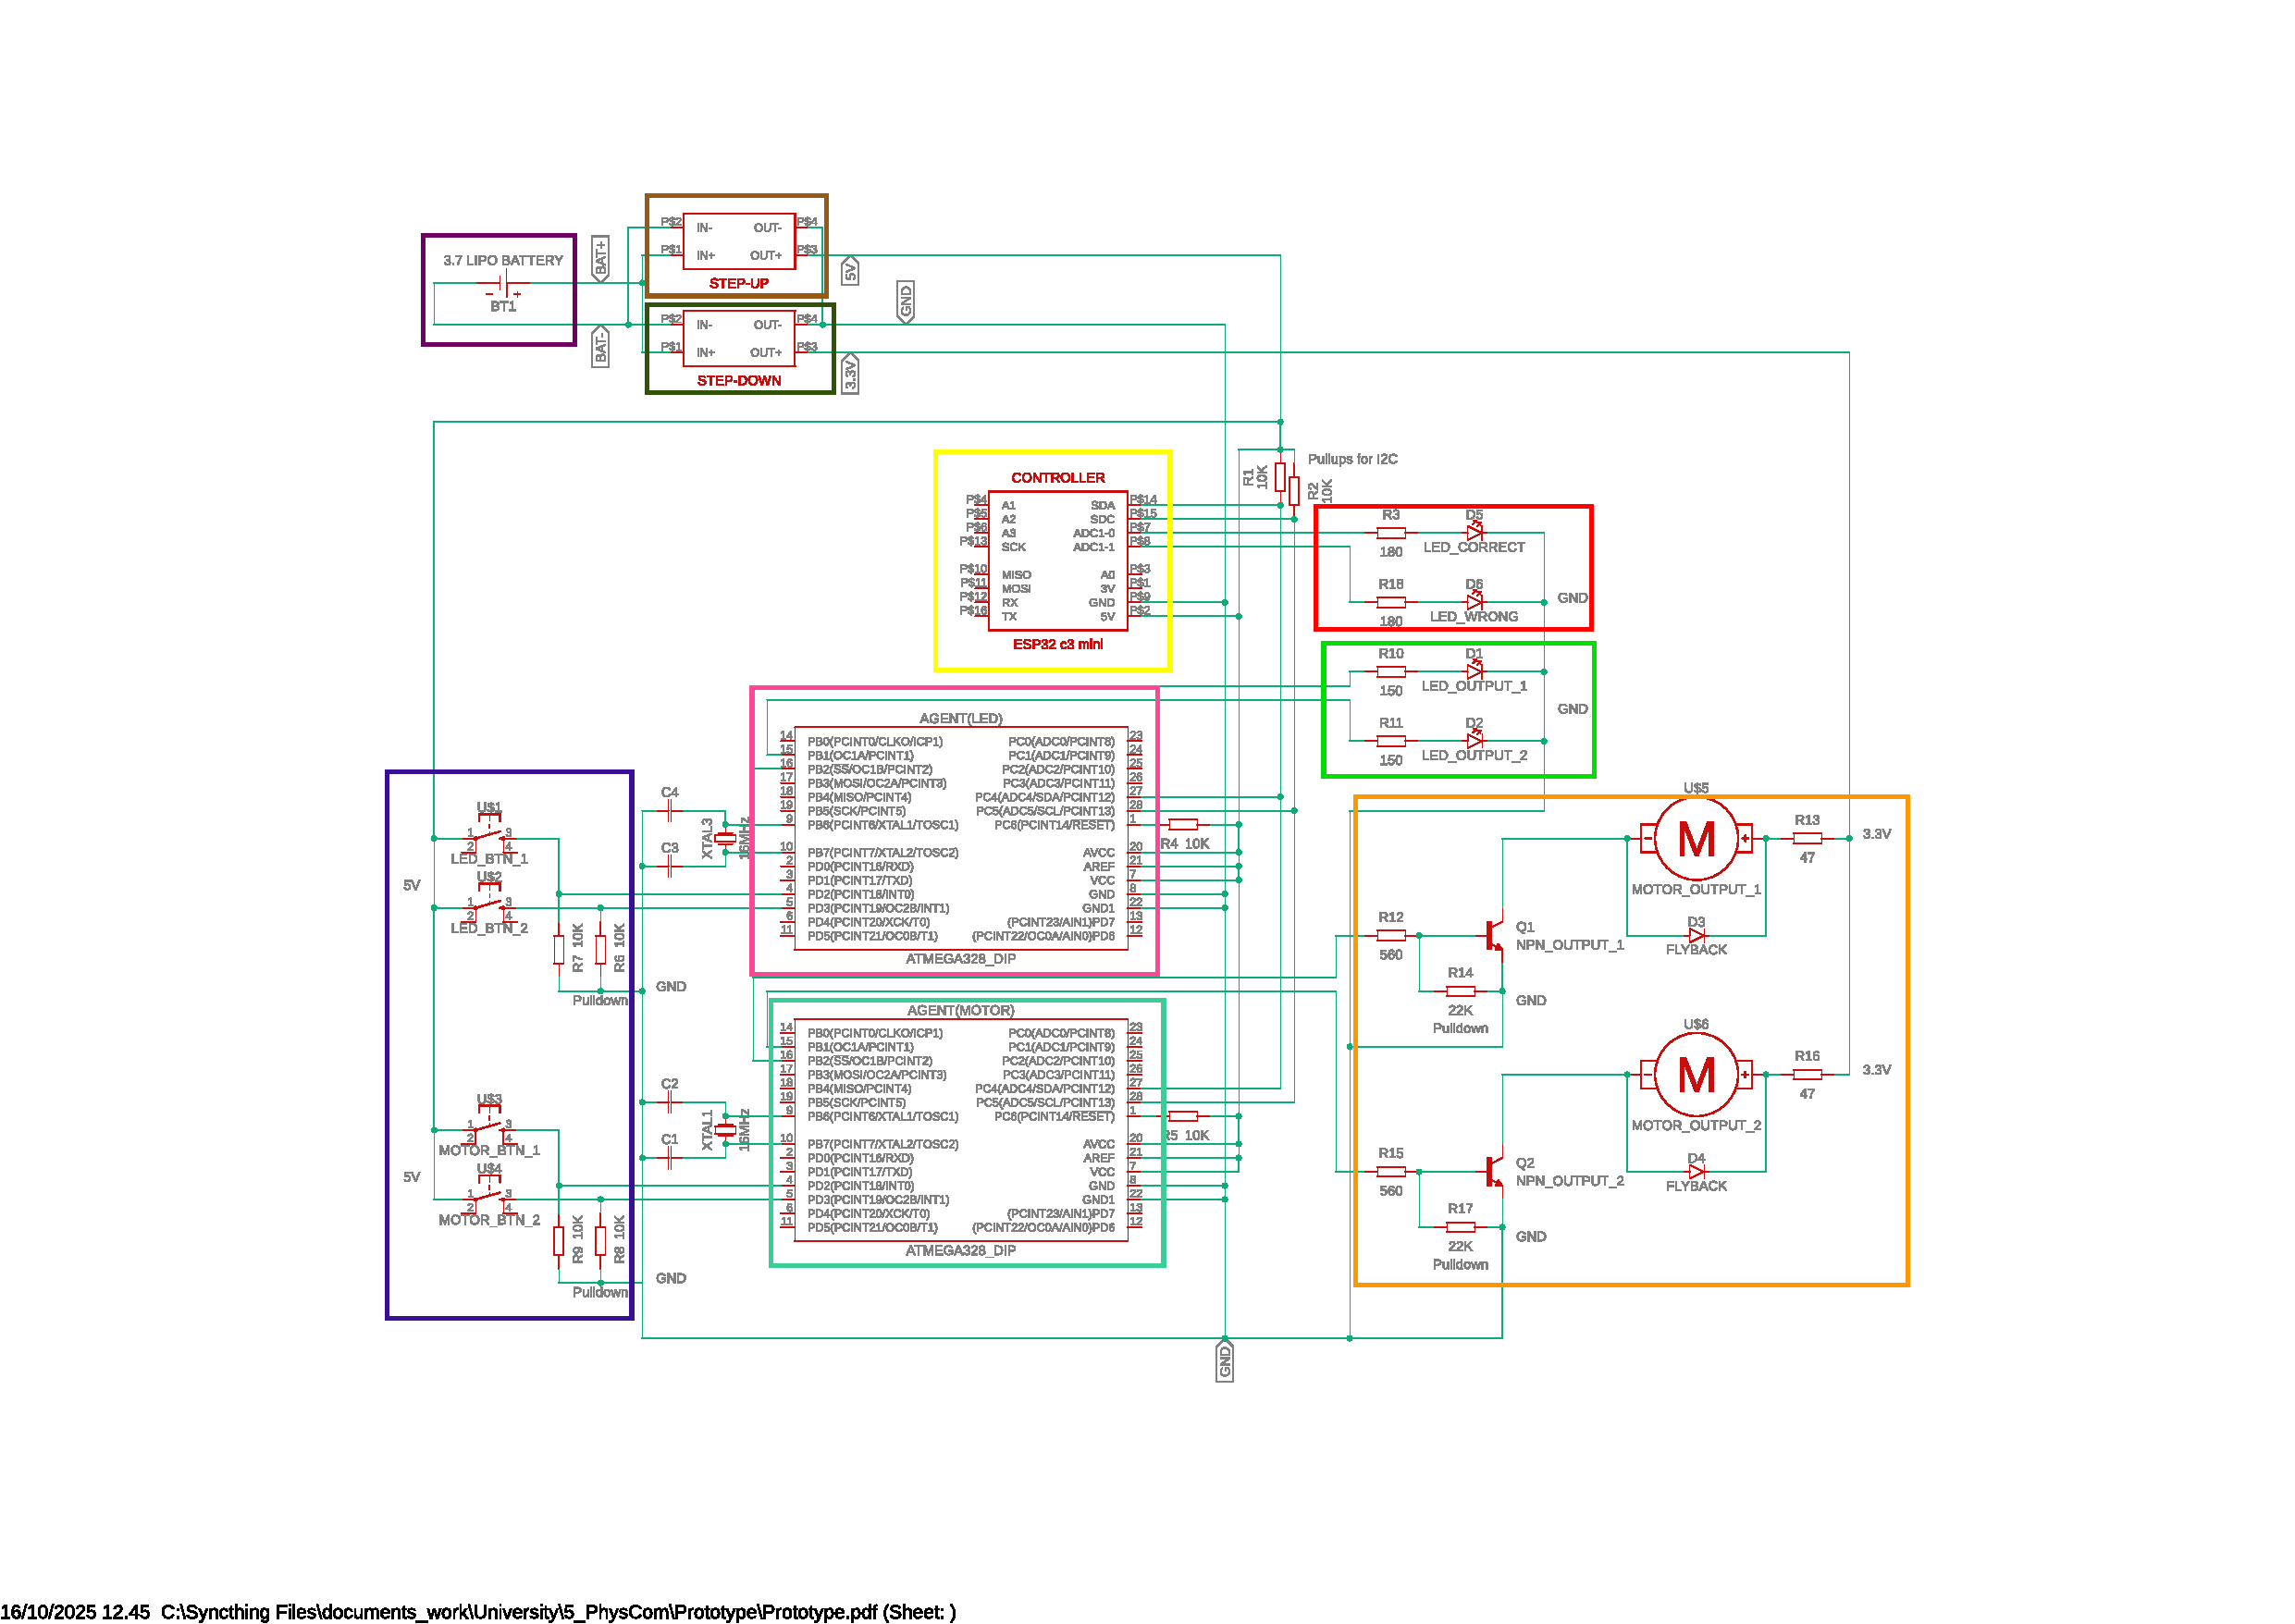
\includepdf[pages=-,landscape,fitpaper=true,pagecommand={}]{img/circuit_diagram_prototype_annotated.pdf}


\subsection{Component Values Calculation}

\subsubsection{LED Resistor Calculation}

V_f := 2V : \\
I_f := 20mA : \\
V_{supply} := 5V : \\
\\
I_f \text{ is the desired current across the resistor (and LED).} \\
V_R \text{ is the voltage across the resistor.} \\
\\
V_R := V_{supply} - V_f = 3V \\
\\
R := \frac{V_R}{I_f} = 150 \Omega
\\
\\

\subsubsection{Motor Resistor calculation}

I_{\max} := 75mA : \\
V_{supply} := 3.3V : \\
R := \frac{V_{supply}}{I_{\max}} = 44.0000000000 \Omega \\
\text{Round up to standard value (47 ohm).}
\\
\\

\subsubsection{BJT Resistor calculation}

\beta_{forced} := 10 : \\
I_C := I_{\max} = 75mA \\
I_B := \frac{I_C}{\beta_{forced}} = \frac{15}{2} mA \text{ at 10 digits} \rightarrow 7.5000000000 mA \\
V_{BE\_sat} := 0.95V \\
V_{supply} := 5V : \\
R := \frac{(V_{supply}) - (V_{BE\_sat})}{I_B} = 540.00000000 \Omega \\

\text{Round up to standard value (560 ohm).}

\subsubsection{References}

\noindent The following websites were used to gather estimate values for components calculation:
\begin{itemize}
\item https://downloads.cree-led.com/files/ds/h/HB-C503B-BAS-BAN-GAS-GAN.pdf
\item https://cdn-shop.adafruit.com/product-files/1201/P1012\_datasheet.pdf
\item https://www.onsemi.com/pdf/datasheet/pzt3904-d.pdf
\end{itemize}


\section{Breadboard Prototype}

\noindent Breadboard prototype for the main setup is shown in figure \ref{fig:main_agents_breadboard} and the power supply for LiPo battery and its voltage conversion in figure \ref{fig:power_supply_breadboard}.

\begin{figure*}[!htb]
  \centering
  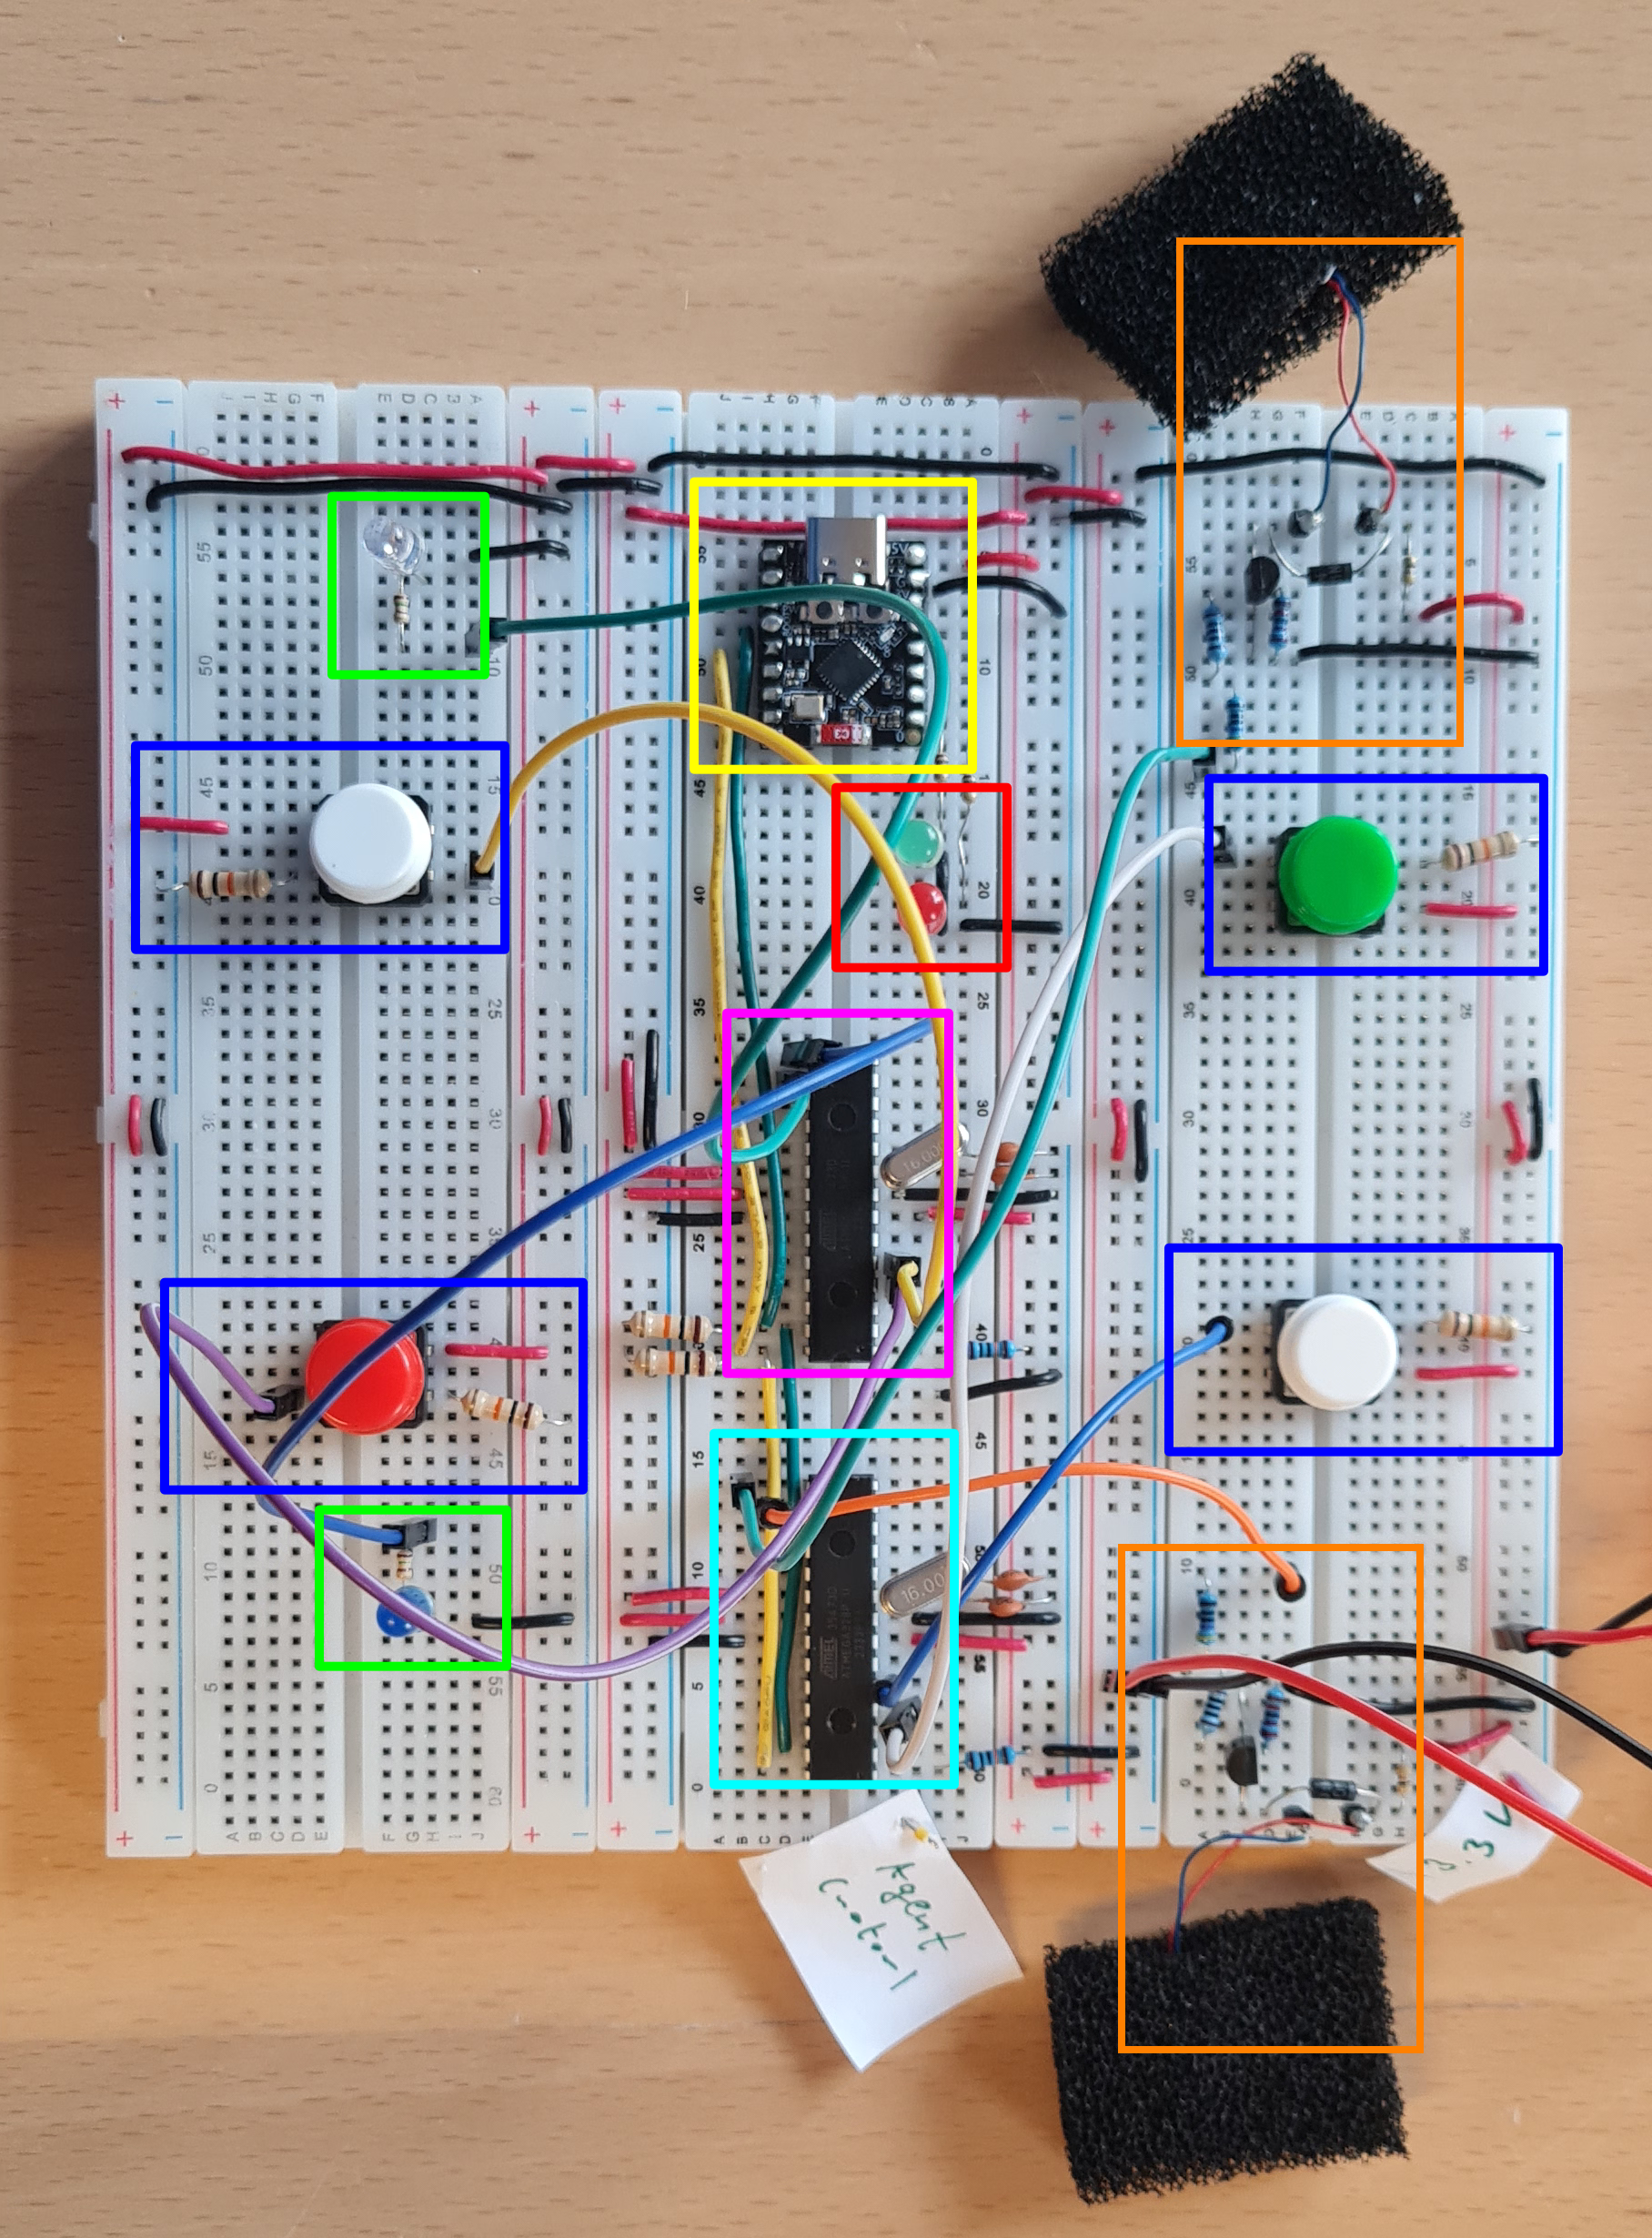
\includegraphics[width=\textwidth]{main_agents_breadboard}
  \caption[Breadboard with main and two agents.]{Breadboard setup of the ESP32 C3 mini main controller and two ATmega agents controlling the motors and LEDs modules.}
  \label{fig:main_agents_breadboard}
\end{figure*}

\begin{figure*}[!htb]
  \centering
  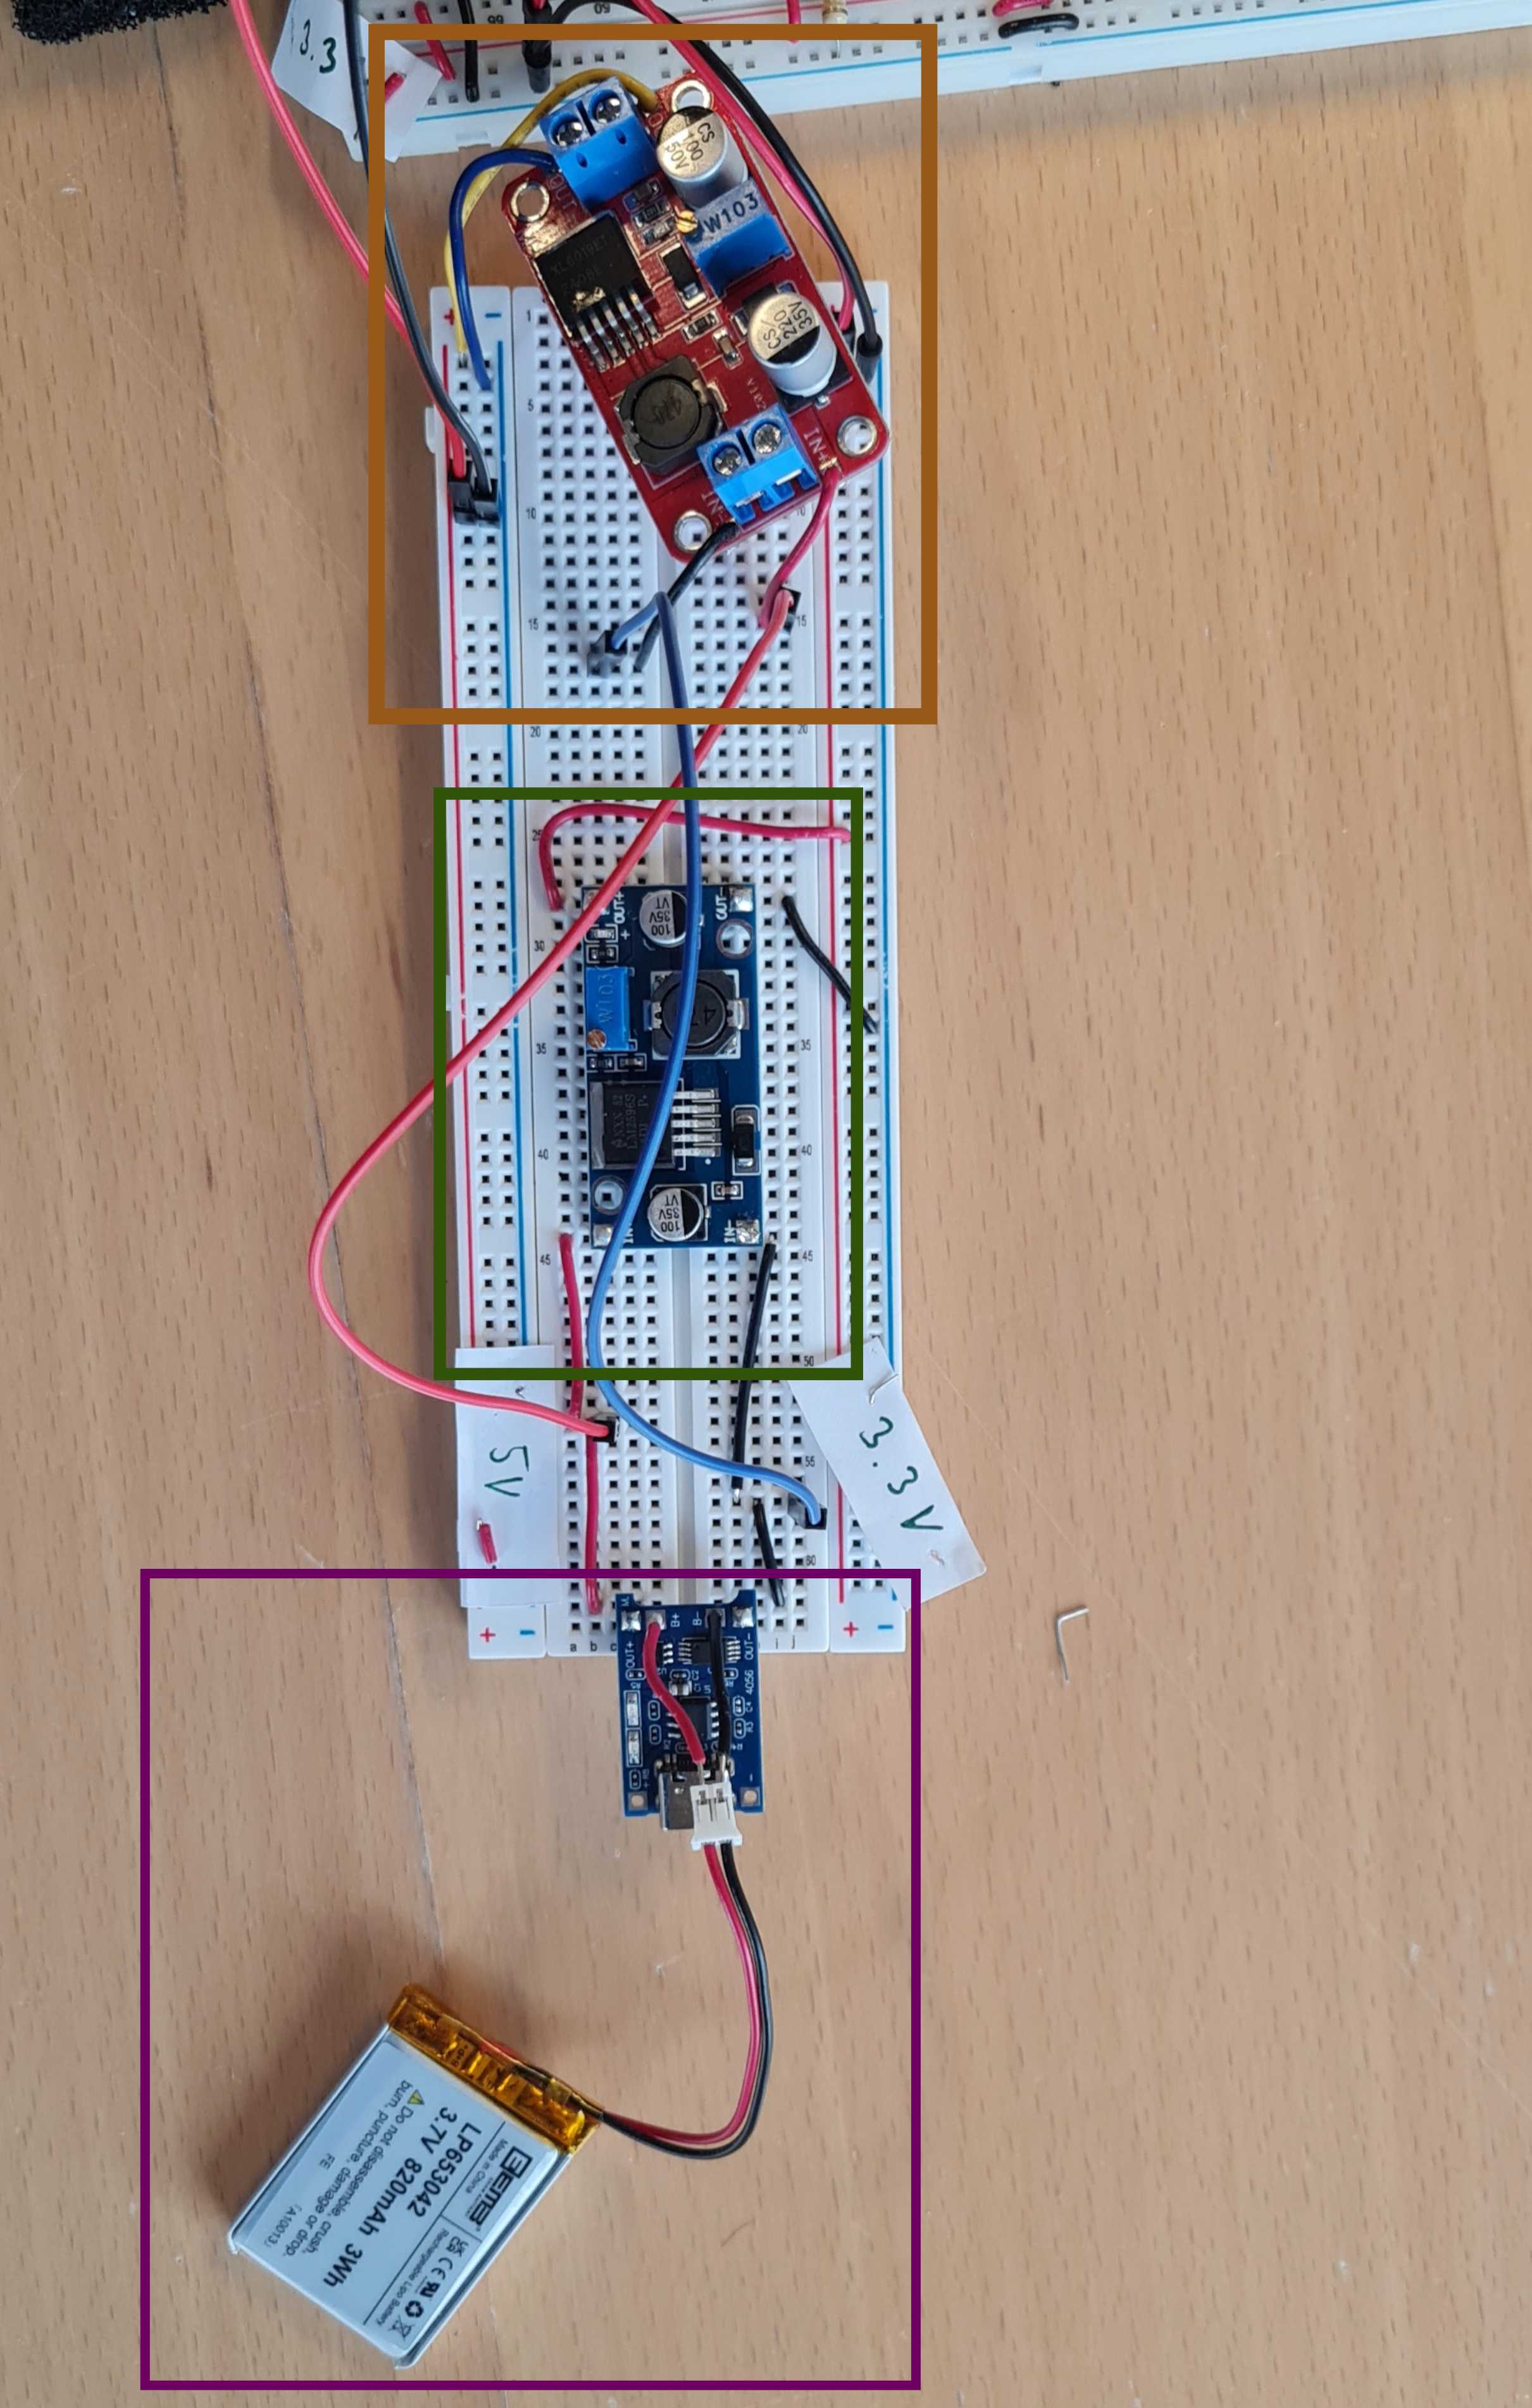
\includegraphics[height=\textheight,keepaspectratio]{power_supply_breadboard}
  \caption[Breadboard with the power supply setup.]{Breadboard setup of the 3.7V battery power supply alongside step-up (to 5V) and step-down (to 3.3V) converters.}
  \label{fig:power_supply_breadboard}
\end{figure*}


\end{document}
